\documentclass[Serif, 10pt, brown]{beamer}
\usepackage{booktabs,xcolor}
%\usepackage[svgnames,table]{xcolor}
%\usepackage[tableposition=above]{caption}
\usepackage{pifont}
\newcommand*\CHECK{\ding{51}}
\usepackage{array}
\newcolumntype{P}[1]{>{\centering\arraybackslash}p{#1}}
%
\usepackage{setspace,mathtools,amssymb,multirow,array,amsmath,tikz}
\usepackage[normalsize]{subfigure}
\usetikzlibrary{patterns}
\usetikzlibrary{automata,positioning,decorations.pathreplacing,decorations}

\usepackage{curves}
\usepackage{wasysym}
\usepackage{epsfig,epstopdf,graphicx}

\curvewarnfalse
%
\newtheorem{proposition}{Proposition}
\theoremstyle{example}
\newtheorem{theoremh}{Theorem}
\theoremstyle{plain}
\renewcommand{\textfraction}{0.01}
\renewcommand{\floatpagefraction}{0.99}
\newcommand{\ul}{\underline}
\newcounter{units}
%
\usepackage[round]{natbib}
 \bibpunct[, ]{(}{)}{,}{a}{}{,}%
 \def\bibfont{\small}%
 \def\bibsep{\smallskipamount}%
 \def\bibhang{24pt}%
 \def\newblock{\ }%
 \def\BIBand{and}%
%
\setbeamercovered{dynamic}
% Logo
\logo{
\includegraphics[width=0.5in,keepaspectratio]{iitb_logo.png}}
%
% Setup
\mode<presentation>
	{
\usetheme[right,currentsection, hideothersubsections]{UTD}
			\useoutertheme{sidebar} \useinnertheme[shadow]{rounded}
			\usecolortheme{whale} \usecolortheme{orchid}
			\usefonttheme[onlymath]{serif}
			\setbeamertemplate{footline}{\centerline{Slide \insertframenumber/\inserttotalframenumber}}
	}
%
% Title
\usebeamercolor[fg]{author in sidebar}
\title[{Approximate Nearest Neighbor Search via Group Testing}]{\sc Approximate Nearest Neighbor Search via Group Testing}
\author[\ul{Authors}]{
  \begin{tabular}{c c c}
    {\bf Saksham Rathi} & {\bf Kshitij Vaidya} & {\bf Ekansh Ravi Shankar} \\
    (22B1003) & (22B1829) & (22B1032)
  \end{tabular}
}
\institute[UTD]{\sc\small CS754: Advanced Image Processing\\ Under Prof. Ajit Rajwade}
\date[UCI]{Indian Institute of Technology Bombay \\ Spring 2025}
%
%Presentation
\begin{document}
\frame{\titlepage}
%
%
%Slides

%TOC

\begin{frame}
	\transblindsvertical
	\frametitle{Contents}
	\tableofcontents[hidesubsections]
\end{frame}
\note[itemize]{
\item Here's the overall structure of my talk today.
}

\section{Introduction}
\begin{frame}{Nearest Neighbor Search}
	\begin{itemize}
		\item Nearest neighbor search is a fundamental problem with many applications in machine learning systems.
		\item {\bf Task:} Given a dataset $D = \{x_1, x_2, \dots , x_N\}$, the goal is to build a data structure that can be queried with any point $q$ to obtain a small set of points $x_i \in D$ that have high similarity (low distance) to the query. This structure is called an index.
		\item Such tasks frequently arise in genomics, web-scale data mining,
		machine learning, and other large-scale applications.
	\end{itemize}
\end{frame}

\begin{frame}{Group Testing}
	\begin{itemize}
		\item We are given a set $D$ of $N$ items, with $k$ positives (“hits”) and $N-k$ negatives (“misses”).
		\item \textbf{Goal:} Identify all positive items using fewer than $N$ group tests.
		\item A \textit{group test} is positive iff at least one item in the group is positive.
		\item \textbf{Testing Variants:} Can be \textit{noisy} (with false positives/negatives), \textit{adaptive} (tests depend on previous results), or \textit{non-adaptive} (all tests run in parallel).
		\item The paper uses a \textbf{doubly regular design:} Each item appears in an equal number of tests; each test has an equal number of items.
	\end{itemize}
\end{frame}

\begin{frame}{Formal Problem Statement}
	\begin{itemize}
		\item \textbf{(R, c)-Approximate Near Neighbor:} Given a dataset $D$, if there exists a point within distance $R$ of a query $y$, return some point within distance $c \cdot R$, with high probability.
		\begin{itemize}
			\item $R$ is the distance threshold (radius).
			\item $c > 1$ is the approximation factor.
		\end{itemize}
		\item Any algorithm that solves the randomized nearest neighbor problem also solves the approximate near neighbor problem with $c=1$ and any $R \ge$ distance to the nearest neighbor.
		\item {(Definition)}
		{\bf Randomized Nearest neighbor:} Given a dataset $D$ and a distance metric $d(\cdot, \cdot)$ and a failure probability $\delta \in [0, 1]$, construct a data structure which, given a query point $y$ reports the point $x \in D$ with the smallest distance $d(x,y)$ with probability greater than $1 - \delta$.
	\end{itemize}
\end{frame}

\section{Locality Sensitive Hashing}

\begin{frame}{Locality Sensitive Hashing}
	A hash function $h(x) \rightarrow \{1, \dots, R\}$ is a function that maps an input $x$ to an integer in the range $[1, R]$. 

	The two points $x$ and $y$ are said to collide if $h(x) = h(y)$.

	\[s(x, y) = Pr_H(h(x) = h(y))\]

	For now, we will assume that $s(x, y) = sim(x, y)$.

	For any positive integer L, we may transform an LSH family $H$ with collision probability $s(x,y)$ into a new family having $s(x,y)^L$ by sampling $L$ hash functions from $H$ and concatenating the values to obtain a new hash code $[h_1(x),h_2(x),...,h_L(x)]$. If the original hash family had the range $[1, R]$, the new hash family has the range $[1, R^L]$.
\end{frame}
\begin{frame}{Locality Sensitive Hashing}
	\begin{itemize}
		\item {\bf Locality Sensitive Hashing (LSH)} algorithms use an LSH function to partition the dataset into buckets.
		\item The hash function is selected so that the distance between points in the same bucket is likely to be small. 
		\item To find the near neighbors of a query, we hash the query and compute the distance to every point in the corresponding bucket.
		\item  {\bf Count-Based LSH} identifies neighbors by simply counting how many times two points land in the same hash bucket across multiple hash functions.
	\end{itemize}
\end{frame}





\section{Distance-Sensitive Bloom Filters}
\begin{frame}{Distance-Sensitive Bloom Filters}
	\begin{itemize}
		\item (Definition) {\bf Approximate Set Membership:} Given a set $D$ of $N$ points and similarity thresholds
		$S_L$ and $S_H$, construct a data structure which, given a query point $y$, has:

		True Positive Rate: If there is $x \in D$ with $sim(x,y) >S_H$, the structure returns true w.p. $ \geq p$

		False Positive Rate: If there is no $x \in D$ with $sim(x,y) > S_L$, the structure returns true w.p. $\leq q$

	\item The distance-sensitive Bloom filter solves this problem using LSH functions and a 2D bit array. The structure consists of $m$ binary arrays that are each indexed by an LSH function. There are threeparameters: the number of arrays $m$, a positive threshold $t \leq m$, and the number of concatenated hash functions $L$ used within each array.  
	\end{itemize}
\end{frame}

\begin{frame}{Distance-Sensitive Bloom Filters}
	\begin{itemize}
		\item To construct the filter, we insert elements $x \in D$ by setting the bit located at array index $[m,h_m(x)]$ to 1. 
		\item To query the filter, we determine the $m$ hash values of the query $y$. If at least $t$ of the corresponding
		bits are set, we return true. Otherwise, we return false. 
		\item (Theorem) Assuming the existence of an LSH family with collision probability $s(x,y) = sim(x,y)$,
		the distance-sensitive Bloom filter solves the approximate membership query problem with
		\[p \geq 1 - exp\left(-2m(-t + S_H^L)^2\right)\]
		\[q \leq exp\left(-2m(-t + NS_L^L)^2\right)\]
	\end{itemize}
\end{frame}

\section{Algorithm}

\begin{frame}{Index Construction}

\textbf{Input:} Dataset $D$ of size $N$, positive integers $B$ and $R$, similarity threshold $S$

\textbf{Output:} A FLINNG search index consisting of membership sets $M_{r,b}$ and group tests $C_{r,b}$

\begin{itemize}
    \item For $r = 0$ to $R - 1$:
    \begin{itemize}
        \item Let $\pi(D)$ be a random permutation of $D$
        \item For $b = 0$ to $B - 1$:
        \begin{itemize}
            \item Define $M_{r,b} = \{ \pi(D)_i \mid i \bmod B = b \}$
        \end{itemize}
    \end{itemize}
    
    \item For $r = 0$ to $R - 1$:
    \begin{itemize}
        \item For $b = 0$ to $B - 1$:
        \begin{itemize}
            \item Construct a classifier $C_{r,b}$ for membership set $M_{r,b}$ with true positive rate $p$ and false positive rate $q$
        \end{itemize}
    \end{itemize}
\end{itemize}
\end{frame}

\begin{frame}{Index Construction}
	\begin{itemize}
		\item If we apply a similarity
		threshold to the dataset, we obtain a near neighbor set $K= \{x \in D | sim(x,y) \geq S\}$. We consider $K$ to be the set of “positives” in the group testing problem.
		\item In order to do so, we split the dataset $D$ into a set of groups, which we visualize as a $B \times R$ grid
		of cells. Each cell has a group of items $M_{r,b}$ and a corresponding group test $C_{r,b}$. To assign items
		to cells, we evenly distribute the $N$ points among the $B$ cells in each column of the grid, and we independently repeat this assignment process $R$ times.
	\end{itemize}
\end{frame}

\begin{frame}{Index Query}
	\textbf{Input:} A FLINNG index and a query $y$

\textbf{Output:} Approximate set $\hat{K}$ of neighbors with similarity greater than the threshold $S$

\begin{itemize}
    \item Initialize $\hat{K} = \{1, \ldots, N\}$
    \item For $r = 0$ to $R - 1$:
    \begin{itemize}
        \item Initialize $Y = \emptyset$
        \item For $b = 0$ to $B - 1$:
        \begin{itemize}
            \item If $C_{r,b}(y) = 1$ then:
            % \begin{itemize}
                $Y = Y \cup M_{r,b}$
            % \end{itemize}
        \end{itemize}
        \item $\hat{K} = \hat{K} \cap Y$
    \end{itemize}
\end{itemize}
\end{frame}

\begin{frame}{Index Query}
	\begin{itemize}
		\item To query the index with a point y, we begin by querying each classifier. If $C_{r,b}(y) = 1$, then at least one of the points in $M_{r,b}$ has high similarity to y. We collect all of these ``candidate points'' by taking the union of the $M_{r,b}$ sets for which $C_{r,b}(y) = 1$. 
		\item We repeat this process for each of the $R$ repetitions to obtain $R$ candidate sets, one for each column in the grid. 
		\item With high probability, each candidate set contains the true neighbors, but it may also have some non-neighbors that were included in $M_{r,b}$ by chance. To filter out these points, we intersect the candidate sets to obtain our approximate near
		neighbor set $\hat{K}$.
	\end{itemize}
\end{frame}

\section{Theory}
\begin{frame}{Group Testing: Runtime and Accuracy}
\textbf{Lemma 1:} Suppose we have a dataset $D$ of points, where a subset $K \subseteq D$ is ``positive'' and the rest are ``negative''. Construct a $B \times R$ grid of tests, where each test has i.i.d true positive rate $p$ and false negative rate $q$. Then the algorithm reports points as ``positive''	with probability:
\[
Pr(\text{Report } x \mid x \in K) \geq p^R
\]
% \[
% Pr(Report x | x \notin K) \leq \left[q\left(\frac{eN(B-1)}{B(N-1)}\right)^{|K|} + p\left(1 - \left(\frac{N(B-1)}{eB(N-1)}\right)^{|K|}\right)\right]^R
% \]

\[
\begin{aligned}
\Pr(\text{Report } x \mid x \notin K) \leq 
\bigg[ q\left(\frac{eN(B-1)}{B(N-1)}\right)^{|K|} 
+ {} & \\
p\left(1 - \left(\frac{N(B-1)}{eB(N-1)}\right)^{|K|}\right) \bigg]^R &
\end{aligned}
\]
\end{frame}

\begin{frame}{Group Testing: Runtime and Accuracy}
	The cost of group testing inference includes the cost to do all $B \times R$ tests, plus the cost of intersecting the positive groups. 

	\textbf{Theorem:} Under the assumptions in the previous lemma, let us suppose that each test runs in $\mathcal{O}(T)$. Then with probability $1 - \delta$:
	\[
	t_{\text{query}} = \mathcal{O}\left(BRT + \frac{RN}{B}(p|K| + qB)log(\frac{1}{\delta})logN\right)
	\]
\end{frame}

\begin{frame}{Bounding the Test Cost}
	To distinguish between the $|K|$ nearest neighbors and the rest of the dataset:
	\[S_H = sim(x_{|K|}, y) = s_{|K|}\]
	\[S_L = sim(x_{|K| + 1}, y) = s_{|K| + 1}\]
	(Definition) $\gamma${\bf -Stable query:} We say that the query is $\gamma$-stable if $\frac{log(s_{|K|})}{log(s_{|K|}) - log(s_{|K|})} \leq \gamma$

	\vspace{0.5cm}
	\textbf{Theorem:} Given a true positive rate p, false negative rate qand stability parameter $\gamma$, it is possible to choose $m$, $L$ and $t$ so that the resulting distance-sensitive Bloom filter has true positive rate $p$ and false negative rate $q$ for all $\gamma$-stable queries. The query time is

	\[\mathcal{O}(mL) = \mathcal{O}(-log(min(q,1-p))N\gamma log(N))\]
\end{frame}


\begin{frame}{Query Time Analysis}
	We will consider the query time of a $2\sqrt{N}\times R$ grid of Bloom filter classifiers and $T = mL$.

	\textbf{Lemma 2:} Under the assumptions of Lemma 1, we can use distance-sensitive Bloom filters as tests to achieve the following query time $t_\text{query}$ of our Algorithm with probability $1 - \delta$

	\[
	\begin{aligned}
		t_\text{query} =
		\mathcal{O}(RN^{\frac{1}{2} + \gamma}log(N) max(-log(q), -log(1-p)) 
	+ {} & \\
	RN^{\frac{1}{2}} log^2(N)(|K|+ qN^{\frac{1}{2}}log(\frac{1}{\delta})) &
	\end{aligned}
	\]

	\textbf{Lemma 3:} Under the assumptions of Lemma 1,we can build a data structure that solves the randomized nearest neighbor problem for sufficiently large N and small $\delta$, where

	$p = 1 - \frac{\delta}{2R}$, $q = N^{-\frac{1}{2}}$, $R = \frac{log(\frac{1}{\delta})}{log(4.80N^{\frac{1}{2}}) - log(2e^2 + 3.44N^{\frac{1}{2}})}$
\end{frame}

\begin{frame}{Query Time Analysis}
	\textbf{Theorem:} Under the assumptions of the previous Lemma, we solve the randomized nearest problem for $\gamma$-stable queries in time $t_\text{query}$:
	\[
		t_\text{query} = \mathcal{O}(N^{\frac{1}{2} + \gamma}log^4(N)log^3(\frac{1}{\delta}))
	\]
	
\end{frame}

% \section{Implementation Details}
% \begin{frame}{Implementation Details}
	
% \end{frame}

\section{Results}
\begin{frame}{Metrics Used}
    \begin{itemize}
        \item \textbf{Query Time (s)}: Measures the total time taken for FLINNG to process the queries. Lower values indicate faster retrieval times.
        \item \textbf{Average Precision}: The fraction of retrieved neighbors that are correct. High precision means most retrieved points are relevant.
        \item \textbf{Average Recall}: The fraction of true nearest neighbors that are retrieved. High recall means most true neighbors are found.
        \item \textbf{F1 Score}: Harmonic mean of precision and recall. A balanced metric that evaluates both correctness and completeness of retrieval.
    \end{itemize}
\end{frame}


\begin{frame}{Default Choice of Parameters}
    \begin{itemize}
        \item \textbf{Dataset Size}: 10,000 points
        \item \textbf{Query Size}: 100 queries
        \item \textbf{Dataset Standard Deviation}: 1
        \item \textbf{Query Standard Deviation}: 0.5
        \item \textbf{Hashes per Table}: 16
        \item \textbf{Number of Hash Tables}: 20
        \item \textbf{k (Nearest Neighbors)}: 1
    \end{itemize}
\end{frame}


\begin{frame}{Heatmap for Query Time}
	\begin{figure}
        \centering
        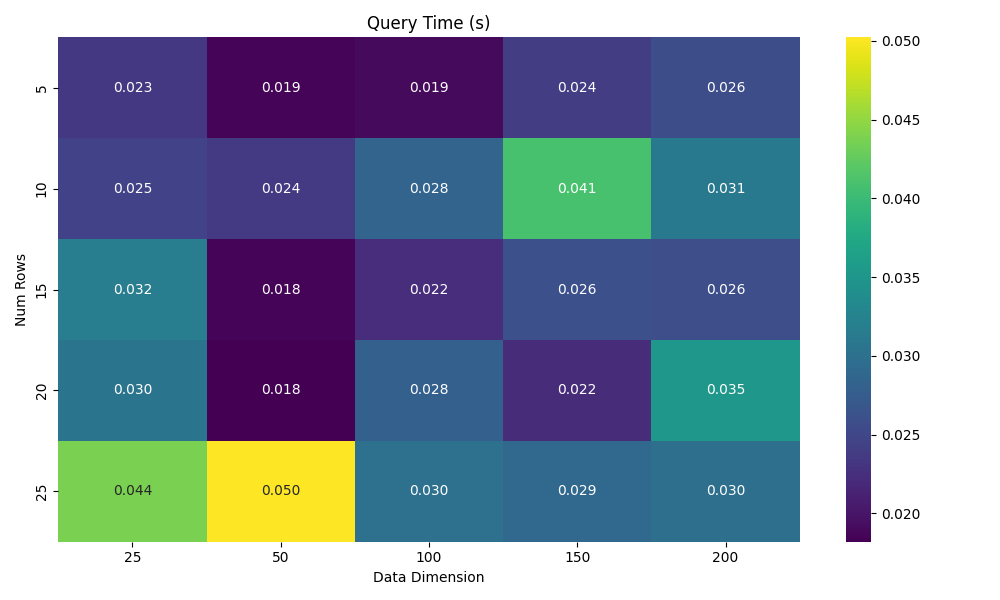
\includegraphics[width=1\linewidth]{../images/query_time_heatmap.png}
    \end{figure}
\end{frame}

\begin{frame}{Heatmap for Average Precision}
	\begin{figure}
		\centering
		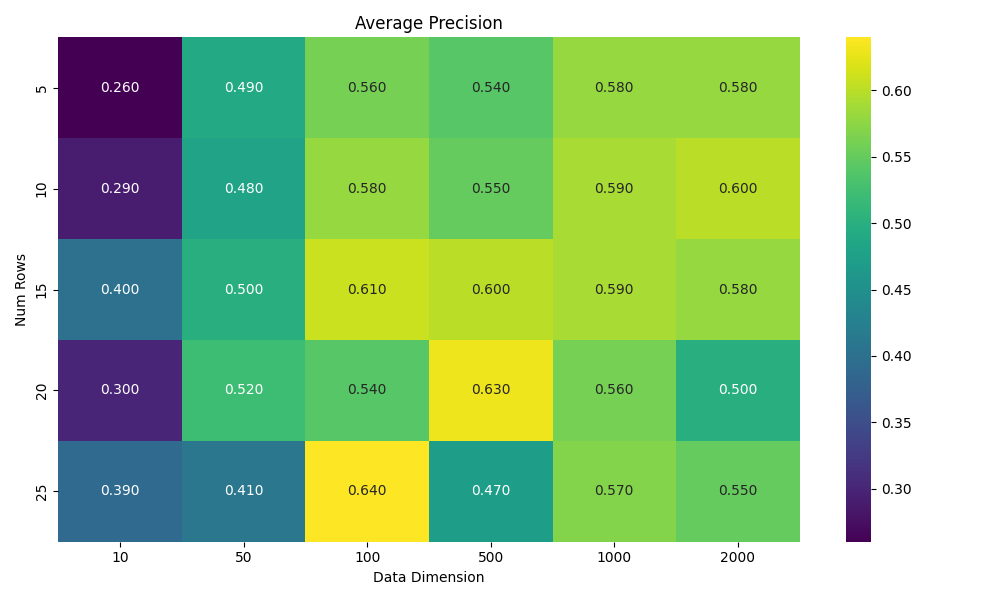
\includegraphics[width=1\linewidth]{../images/precision_heatmap.png}
	\end{figure}
\end{frame}

\begin{frame}{Heatmap for Average Recall}
	\begin{figure}
		\centering
		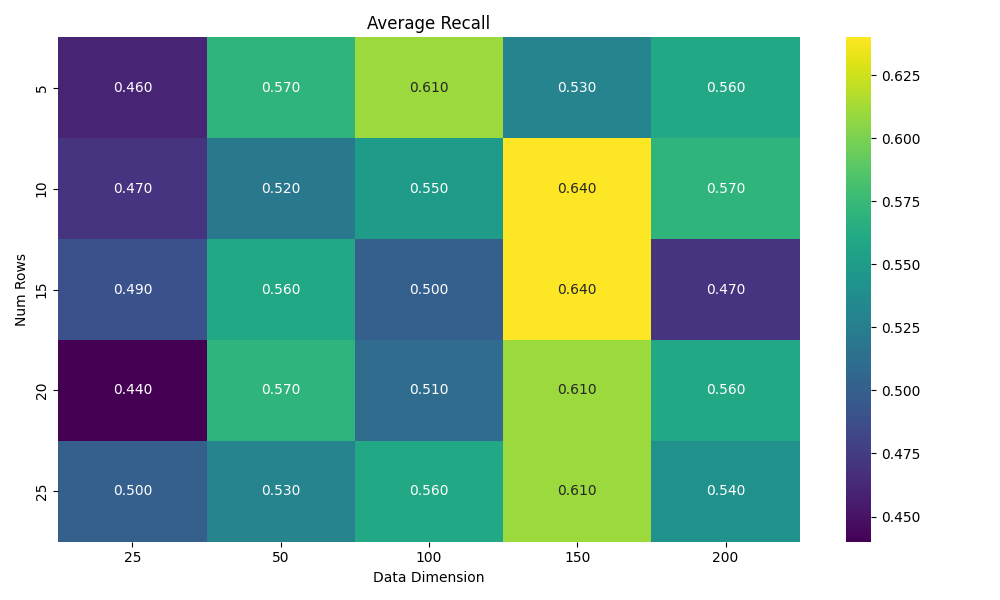
\includegraphics[width=1\linewidth]{../images/recall_heatmap.png}
	\end{figure}
\end{frame}

\begin{frame}{Heatmap for Average F1 Score}
	\begin{figure}
		\centering
		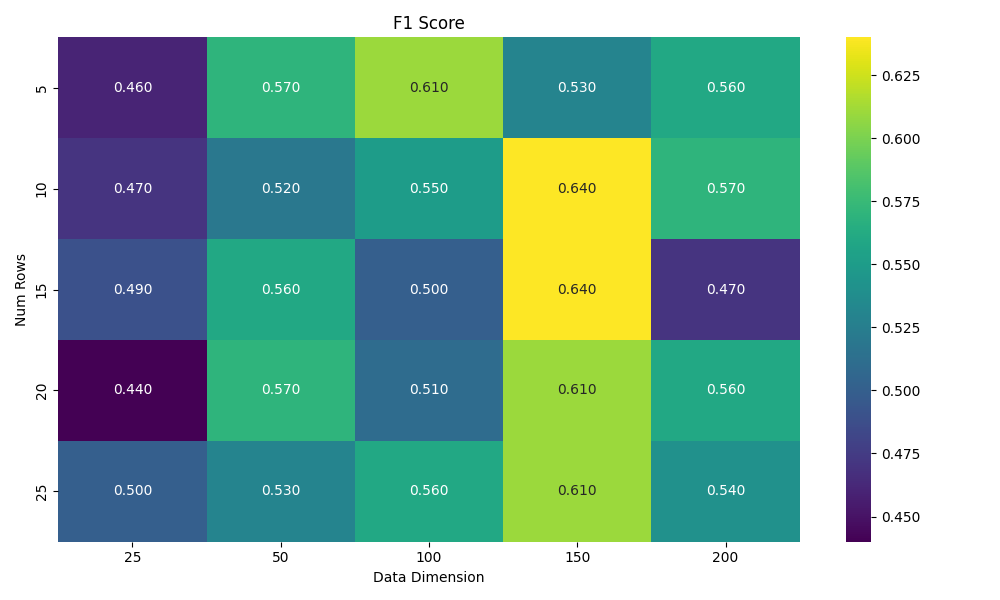
\includegraphics[width=1\linewidth]{../images/f1_score_heatmap.png} 
	\end{figure}
\end{frame}

\begin{frame}{Individual Contributions}
	\begin{itemize}
		\item \textbf{Saksham Rathi}: Read through the paper, described the initial problem statement and the algorithms used in the paper in the report, code debugging, collection of results and adding them to the report.
		\item \textbf{Kshitij Vaidya}: Read through the paper, wrote the LSH, DSBF and FLINNG classes in Python and tested them for correct functionality, code debugging.
		\item \textbf{Ekansh Ravi Shankar}: Read through the paper, code debugging, wrote threshold relaxation algorithm.
	\end{itemize}
	
\end{frame}


\begin{frame}{Code and Report}
    The code and the report can be found at the following link:
    \begin{center}
        \url{https://github.com/sakshamrathi21/CS754-Project}
    \end{center}
\end{frame}

\begin{frame}
    \Huge{\centerline{\bf Thank You}}
\end{frame}






\end{document}